\section{Безопасность в статистических БД}

\subsection{Определение статистической базы данных}

Статистическая база данных — это специализированный тип базы данных, который разработан и оптимизирован для хранения и управления статистическими данными. Она представляет собой совокупность таблиц, где каждая таблица содержит переменные (столбцы), представляющие различные характеристики или атрибуты, и наблюдения (строки), представляющие отдельные единицы данных или объекты. Статистические базы данных часто содержат большие объемы данных, собранных из различных источников, таких как опросы, эксперименты, наблюдения и административные записи. Такие базы данных могут содержать разнообразные типы данных, включая числовые, категориальные, временные ряды и многие другие. Они могут быть созданы и использованы для различных целей, таких как проведение исследований, анализ данных, подготовка отчетов, прогнозирование и принятие решений.
\\

Статистические базы данных обычно имеют стандартизированную структуру и формат, чтобы обеспечить согласованность и удобство использования данных для статистического анализа. Они также могут включать механизмы для обновления данных, контроля качества данных и обеспечения конфиденциальности и безопасности информации.
\\

\subsection{Классификация статистических баз данных}
Основные характеристики статистических баз данных включают:
\begin{enumerate}
    \item \textbf{Структуру данных:} статистические базы данных имеют четко определенную структуру, которая организует данные в таблицы, где каждая таблица представляет конкретную сущность данных или переменную. Структура включает поля (столбцы), представляющие различные атрибуты или характеристики, и записи (строки), представляющие отдельные экземпляры данных.
    \item \textbf{Интеграцию данных:} статистические базы данных могут интегрировать данные из нескольких источников для создания комплексного набора данных для анализа. Этот процесс интеграции включает сопоставление и преобразование данных для обеспечения согласованности и совместимости.
    \item \textbf{Качество данных:} обеспечение качества данных имеет важное значение в статистических базах данных. Они используют механизмы проверки данных, их очистки и стандартизации для минимизации ошибок, несогласованностей и пропущенных значений, которые могут повлиять на достоверность статистического анализа.
    \item \textbf{Метаданные:} статистические базы данных часто включают метаданные, которые содержат информацию о данных, такую как определения переменных, источники данных, методы сбора данных и любые преобразования, примененные к данным.
    \item \textbf{Политики безопасности и конфиденциальности:} статистические базы данных работают с конфиденциальными данными, такими как информация о персональных данных, банковские данные, бухгалтерские ведомости и подобными, и поэтому должны иметь меры безопасности для защиты конфиденциальности. Часто используются контроль доступа и методы анонимизации для обеспечения конфиденциальности данных.
\end{enumerate}


Статистические базы данных служат ценным ресурсом для исследователей, аналитиков и принимающих решения. Они позволяют выполнять различные статистические операции, такие как агрегирование, корреляция, регрессия и проверка гипотез, для выявления паттернов, взаимосвязей и тенденций в данных.
\\

Статистические базы данных позволяют проводить анализ данных, отвечать на исследовательские вопросы и принимать информированные решения на основе фактов. Они являются основой для множества статистических исследований, позволяя исследователям изучать различные явления, разрабатывать статистические модели и предсказывать будущие события.
\\

Примеры статистических баз данных могут включать базы данных национальных статистических агентств, таких как Федеральное агентство по статистике (Росстат) или Бюро экономического анализа (BEA) в США. Эти базы данных содержат широкий спектр статистической информации о населении, экономике, здравоохранении, социальных показателях и других аспектах жизни.
\\

Важно отметить, что статистические базы данных могут иметь различные спецификации и структуры, в зависимости от конкретной области знаний и целей использования данных.

\subsection{Задача безопасности статических баз данных}
Следующие 4 раздела являются переводом статьи \cite{brankovic2007statistical}.
Безопасность статистических баз данных связана с защитой конфиденциальности лиц, чьи конфиденциальные данные собираются посредством опросов или других средств, и
используется для облегчения статистических исследований. 
\\

Самым ранним примером статистических баз данных, несомненно, являются данные переписи населения,
сбор, хранение и анализ которой претерпели большие изменения
за последние 6000 лет. Помимо переписи, статистические центры 
в различных странах также собирают множество других видов данных, как правило, посредством опросов, а затем обрабатывают и распространяют данные многочисленным другим организациям и органам. Более того, многие организации начали собирать свои собственные данные либо для собственных исследований, стратегического планирования, маркетинга, либо с намерением продать его другим заинтересованным лицам. Неудивительно, что этот массовый сбор и обмен данными усилил и без того растущую обеспокоенность общественности по поводу неправомерного использования и несанкционированного раскрытия конфиденциальной индивидуальной информации.
\\

В контексте этой главы будем называть \textit{владельцем данными} человека, который собирает данные и управляет ими.
В настоящее время перед владельцами данных стоит очень сложная задача - получить и предоставить
пользователям данные и неограниченный доступ к статистике, но в то же время обеспечить распространение данных таким образом, чтобы исключить возможность идентификации конкретных людей. Этот процесс часто известен как контроль за статистическим раскрытием (statistical disclosure control) или обеспечение безопасности статистических баз данных.
\\

Существует две основные группы методов контроля статистического раскрытия, которые могут быть использованы для защиты конфиденциальности, а именно, методы ограничения и методы добавления шума. Методы ограничения ограничивают информацию, доступную пользователю, либо напрямую, либо через ответы на их запросы. Однако вся доступная информация точна. С другой стороны, методы добавления шума сохраняют доступность данных, но не их точность. Другими словами, все данные доступны, но они только приблизительны, так как прошли через процесс искажения перед предоставлением пользователю. Оба метода имеют свои преимущества и недостатки, и может быть необходимо применять их одновременно для обеспечения необходимого уровня конфиденциальности. Кроме этих двух методов, конфиденциальность также может быть защищена с использованием безопасных вычислений между несколькими сторонами (secure multiparty computations).
\\

\subsection{Основные понятия}
В этом разделе мы подробно рассмотрим абстрактную модель статистических базы данных, введем некоторые важные понятия из теории статистических баз данных и проиллюстрируем их на нашем рабочем примере.
\\

В таблице \ref{tab:main} представлены данные, которые могут входить в базу данных переписи населения. Разумеется, это всего лишь игрушечный пример, помогающий нам проиллюстрировать некоторые понятия. Реальная перепись населения в большинстве стран обычно содержит миллионы записей и десятки переменных.
\\

В абстрактной модели статистическая база данных представляет собой двумерную таблицу, где каждая строка описывает индивида, будь то человек, предприятие или какая-то другая сущность. В нашем примере базы данных переписи каждая строка описывает главу семейства и несколько свойств его семьи: \textit{КВ} (\textit{КД}) - количество взрослых (детей), \textit{ДС} - доход семьи, в то время как стобец \textit{Доход} - доход главы семейства, \textit{ВЖ} - владение каким-либо жильем, \textit{ПР} - потребность в ремонте жилья. Следуя терминологии баз данных, мы называем эти свойства \textit{атрибутами}. В таблице ГС означает главу семейства. Каждому атрибуту сопоставлен домен, то есть набор допустимых значений, которые атрибут может принимать. Например, в нашей базе данных доменом атрибута \enquote{КД} является множество неотрицательных целых чисел.
\\

\begin{table}[]
\small
\begin{tabular}{|c|c|c|c|c|c|c|c|c|c|c|}

\hline
   & Адрес     & Имя             & Пол & Доход & Возраст & КВ & КД & ДС & ВЖ & ПР \\ \hline
1  & ул. Пролетарская, 13 & Анна Шустова       & Ж      & 70       & 34         & 1                   & 1                & 70          & Да              & Нет                   \\ \hline
2  & ул. Ленина, 32       & Александр Иванов   & М      & 99       & 39         & 2                   & 2                & 99          & Да              & Да                    \\ \hline
3  & ул. Мира, 4          & Екатерина Новикова & Ж      & 33       & 21         & 1                   & 0                & 33          & Да              & Нет                   \\ \hline
4  & ул. Гагарина, 88     & Дмитрий Смирнов    & М      & 21       & 21         & 1                   & 0                & 21          & Да              & Да                    \\ \hline
5  & ул. Советская, 42    & Иван Жаров        & М      & 21       & 27         & 2                   & 1                & 40          & Да              & Да                    \\ \hline
6  & ул. Пушкина, 65      & Мария Петрова      & Ж      & 55       & 38         & 3                   & 2                & 110         & Нет             & Нет                   \\ \hline
7  & ул. Жукова, 56       & Ольга Полежайкина     & Ж      & 84       & 51         & 1                   & 1                & 84          & Да              & Да                    \\ \hline
8  & ул. Кирова, 17       & Татьяна Морозова   & Ж      & 67       & 35         & 2                   & 3                & 100         & Нет             & Нет                   \\ \hline
9  & ул. Московская, 21   & Сергей Соколов     & М      & 23       & 44         & 2                   & 2                & 50          & Да              & Да                    \\ \hline
10 & ул. Строителей, 1    & Андрей Жилин     & М      & 34       & 28         & 2                   & 3                & 34          & Нет             & Да                    \\ \hline
11 & ул. Садовая, 77      & Михаил Цаплев      & М      & 45       & 47         & 2                   & 1                & 45          & Нет             & Нет                   \\ \hline
12 & ул. Лесная, 37       & Владимир Царев    & М      & 12       & 60         & 1                   & 0                & 12          & Да              & Да                    \\ \hline
13 & ул. Центральная, 44  & Наталья Волкова    & Ж      & 56       & 33         & 2                   & 2                & 70          & Да              & Да                    \\ \hline
14 & ул. Первомайская, 82 & Ирина Козлова      & Ж      & 23       & 31         & 2                   & 3                & 45          & Да              & Да                    \\ \hline
\end{tabular}
\caption{База данных для переписи населения для города Х}
\label{tab:main}
\end{table}

Атрибуты в статистической базе данных могут быть либо конфиденциальными, либо неконфиденциальными, иногда также называемыми идентификаторами и чувствительными атрибутами, соответственно. В базе данных переписи, вероятно, неконфиденциальными атрибутами будут адрес, имя и пол главы семейства, количество взрослых и детей в семье. Остальные атрибуты считаются конфиденциальными. Неконфиденциальные атрибуты являются общедоступными знаниями и, вероятно, известны нарушителю. Эти атрибуты могут быть использованы для идентификации отдельных записей. Некоторые атрибуты могут идентифицировать записи напрямую и называются \textit{прямыми идентификаторами}. В базе данных переписи адрес и имя главы семейства действуют как прямые идентификаторы. Другие могут идентифицировать записи только в сочетании с другими атрибутами и называются \textit{косвенными идентификаторами}. Подмножество косвенных идентификаторов, которые могут использоваться вместе для идентификации записей, называется \textit{ключом}, также известным как \textit{квази-идентификатор}. 
\\

Обратите внимание, что есть важное различие между ключом в теории баз данных и нашим ключом здесь: в теории баз данных ключ - это комбинация атрибутов, которая однозначно идентифицирует каждую запись в базе данных. Другими словами, нет двух записей с одинаковыми значениями всех атрибутов ключа. В нашем контексте некоторые значения ключа могут уникально идентифицировать запись, а другие - нет. Например, в нашем примере (Пол, КВ, КД) действуют вместе как ключ. Запись 13 однозначно идентифицируется значением ключа (Ж, 2, 2). Однако значение ключа (M, 2, 2) совпадает как с записью 2, так и с записью 9, и, следовательно, (Пол, КВ, КД) не подходит в качестве ключа в базовом понимании баз данных. 
\\

Из этого концепта ключа (квази-идентификатора) возникает свойство k-анонимности. Мы говорим, что база данных обеспечивает \textit{k-анонимность}, если для каждой комбинации значений ключа в k-анонимной базе данных есть по крайней мере k записей, которые разделяют эти значения.
\\

Первым логическим шагом в защите конфиденциальности в статистической базе данных было бы удалить все прямые идентификаторы, что обычно делается на практике перед распространением данных. Однако было бы неверно предположить, что этот шаг в одиночку достаточен для истинной анонимизации данных. Большой процент записей, особенно в небольших базах данных, по-прежнему могут быть идентифицированы с использованием ключей, состоящих из косвенных идентификаторов. В этом случае следует применить один из методов, описанных в следующих двух разделах. Также база данных может быть выпущена в виде сводных таблиц, что позволит скрыть некоторую информацию. Таблица \ref{tab:summain} - пример такой двумерной таблицы. 

\begin{table}[h]
\centering
\begin{tabular}{|c|cccccc|}
\hline
                        & \multicolumn{6}{c|}{КД}                                                                                                         \\ \hline
\multirow{4}{*}{Пол} & \multicolumn{1}{c|}{}      & \multicolumn{1}{c|}{0}  & \multicolumn{1}{c|}{1}   & \multicolumn{1}{c|}{2}   & \multicolumn{1}{c|}{3}   & Всего \\ \cline{2-7} 
                        & \multicolumn{1}{c|}{М}     & \multicolumn{1}{c|}{33} & \multicolumn{1}{c|}{85}  & \multicolumn{1}{c|}{149} & \multicolumn{1}{c|}{34}  & 334   \\ \cline{2-7} 
                        & \multicolumn{1}{c|}{Ж}     & \multicolumn{1}{c|}{33} & \multicolumn{1}{c|}{154} & \multicolumn{1}{c|}{180} & \multicolumn{1}{c|}{145} & 479   \\ \cline{2-7} 
                       & \multicolumn{1}{c|}{Всего} & \multicolumn{1}{c|}{66} & \multicolumn{1}{c|}{239} & \multicolumn{1}{c|}{329} & \multicolumn{1}{c|}{179} & 813   \\ \hline
\end{tabular}
\caption{Таблица доходов семей для атрибутов \enquote{Пол} и \enquote{КД}}
\label{tab:summain}
\end{table}

\subsection{Метод ограничения}
Техники, ограничивающие статистику, обычно можно разделить на три основные категории: глобальное перекодирование, подавление и ограничение запросов. Цель глобального перекодирования и подавления заключается в устранении редких комбинаций значений атрибутов ключа, то есть комбинаций, которые встречаются либо в одной записи, либо в небольшом количестве записей. Обычно сначала применяется глобальное перекодирование для устранения большинства редких комбинаций, а затем подавление, чтобы устранить оставшиеся случаи.
\\

Глобальное перекодирование (ГП) трансформирует область атрибута. Если атрибут является категориальным, то ГП подразумевает схлопывание нескольких категорий в одну. Для числовых атрибутов ГП определяет диапазоны значений и затем заменяет каждое отдельное значение его соответствующим диапазоном. Например, чтобы устранить редкие комбинации значений косвенных идентификаторов в нашем примере, мы могли бы заменить области \enquote{КВ} и \enquote{КД} диапазонами \enquote{0 или 1} и \enquote{2 или более}.
\\

ГП также может быть применено к данным, представленным в виде сводных таблиц, в котором случае это называется переработкой таблицы или схлопыванием строк или столбцов. Например, в таблице \ref{tab:summain} ячейка (1,4), описывающая общий доход всех семей с тремя детьми и главой семьи мужчиной, чувствительна, так как существует только одна такая семья в исходной таблице (запись 10). Точно так же ячейка (2,1) чувствительна, так как также содержит только одну семью (запись 3). Чтобы устранить чувствительные ячейки, таблицу можно переработать, схлопнув значения \enquote{КД} 0 и 1 в единую категорию \enquote{0 или 1}, а значения 2 и 3 в единую категорию \enquote{2 или более}. Новая сводная таблица представлена в таблице \ref{tab:GP}.
\\

\begin{table}[h]
\centering
\begin{tabular}{|c|cccc|}
\hline
                        & \multicolumn{4}{c|}{КД}                                                                \\ \hline
\multirow{4}{*}{Пол} & \multicolumn{1}{c|}{}      & \multicolumn{1}{c|}{0 или 1} & \multicolumn{1}{c|}{2 или более} & Всего \\ \cline{2-5} 
& \multicolumn{1}{c|}{М}     & \multicolumn{1}{c|}{118}     & \multicolumn{1}{c|}{183}         & 334   \\ \cline{2-5} 
                        & \multicolumn{1}{c|}{Ж}     & \multicolumn{1}{c|}{187}     & \multicolumn{1}{c|}{325}         & 479   \\ \cline{2-5} 
                        & \multicolumn{1}{c|}{Всего} & \multicolumn{1}{c|}{305}     & \multicolumn{1}{c|}{508}         & 813   \\ \hline
\end{tabular}
\caption{Таблица доходов семей для атрибутов \enquote{Пол} и \enquote{КД} после глобального перекодирования}
\label{tab:GP}
\end{table}

Подавление заменяет значение атрибута в одной или нескольких записях на пропущенное значение. Важно отметить, что в случае сводных таблиц обычно недостаточно подавить чувствительные ячейки. Например, если в таблице \ref{tab:summain} мы подавим две чувствительные ячейки, (1,4) и (2,1), злоумышленник все равно сможет вывести их значения. Ему просто нужно будет вычесть значения всех остальных ячеек в соответствующей строке (столбце) из общего итога для этой строки (столбца). Таким образом, нам нужно подавить как минимум 2 ячейки в каждой строке (столбце), на которую влияет подавление. Таблица \ref{tab:suppression} показывает пример минимального количества подавлений, которые нам нужно выполнить - в данном случае четыре. Эти дополнительные подавления называются вторичными подавлениями. При выборе ячеек для вторичного подавления должны быть выполнены следующие три требования. Во-первых, ни одна пустая ячейка не должна быть подавлена. Сначала можно применить переработку таблицы, чтобы устранить или минимизировать пустые и чувствительные ячейки. Во-вторых, для минимизации потери информации общее количество подавленных ячеек должно быть как можно меньше. После вторичного подавления злоумышленник все равно сможет определить диапазон выполнимости для каждой подавленной ячейки. Например, из таблицы  можно заключить, что значение для ячейки (4,1) находится в диапазоне [1,67]. Третьим требованием, которому должно удовлетворять вторичное подавление, является то, что диапазоны выполнимости не должны быть слишком узкими.
\\

\begin{table}[h]
\centering
\begin{tabular}{|c|cccccc|}
\hline
                        & \multicolumn{6}{c|}{КД}                                                                                                         \\ \hline
\multirow{4}{*}{Пол} & \multicolumn{1}{c|}{}      & \multicolumn{1}{c|}{0}  & \multicolumn{1}{c|}{1}   & \multicolumn{1}{c|}{2}   & \multicolumn{1}{c|}{3}   & Всего \\ \cline{2-7} 
                        & \multicolumn{1}{c|}{М}     & \multicolumn{1}{c|}{X} & \multicolumn{1}{c|}{85}  & \multicolumn{1}{c|}{149} & \multicolumn{1}{c|}{X}  & 334   \\ \cline{2-7} 
                        & \multicolumn{1}{c|}{Ж}     & \multicolumn{1}{c|}{X} & \multicolumn{1}{c|}{154} & \multicolumn{1}{c|}{180} & \multicolumn{1}{c|}{X} & 479   \\ \cline{2-7} 
                        & \multicolumn{1}{c|}{Всего} & \multicolumn{1}{c|}{66} & \multicolumn{1}{c|}{239} & \multicolumn{1}{c|}{329} & \multicolumn{1}{c|}{179} & 813   \\ \hline
\end{tabular}
\caption{Таблица доходов семей для атрибутов \enquote{Пол} и \enquote{КД} после подавления}
\label{tab:suppression}
\end{table}

Третий тип техник ограничения - так называемое ограничение запросов. Запрошенные пользователем запросы либо отвечаются точно, либо отвергаются. Решение о том, на какие запросы ответить, принимается с использованием одной из следующих техник: новый запрос отвечается только в том случае, если вместе со всеми ранее отвеченными запросами он не приводит к компрометации. 
\\

\subsection{Метод добавления шума}

Основная идея любой техники добавления шума (ДШ) заключается в маскировке истинных значений чувствительных данных путем добавления к ним определенного уровня ошибки. Это делается контролируемым образом с целью наилучшего баланса между конкурирующими потребностями в конфиденциальности и потерей информации. Введение шума в выпущенную статистику делает задачу обеспечения качества статистических анализов сложной. Однако есть преимущества использования методов ДШ, одним из которых является их относительная легкость внедрения и низкие эксплуатационные расходы.
\\

Техники ДШ могут быть классифицированы несколькими способами. Один из способов - по типу атрибута, к которому они могут быть применены. Мы говорим, что атрибут является \textit{числовым}, если его значения имеют естественный порядок, независимо от того, являются ли значения фактически числами или нет, и \textit{категориальным} в противном случае. Техники также могут быть классифицированы в зависимости от того, как шум добавляется. Он может быть добавлен перед выпуском статистики, в котором случае исходная база данных обычно заменяется искаженной базой данных, на которой выполняются статистические запросы. Этот тип метода обычно известен как подход к искажению данных. Для техник выдачи шума запросы оцениваются на исходных данных, и к результатам таких запросов добавляется шум.
\\

\subsection{Проблемы безопасности персональных данных в статистических базах данных}

Статистической (в приведенном в этом разделе контексте) считается база данных, в которой допускаются запросы с обобщением данных (суммированием, вычислением среднего значения и т.д.), но не допускаются запросы по отношению к элементарным данным. Например, в статистической базе данных разрешается выдача запроса \enquote{Какова средняя зарплата программистов?} тогда как выдача запроса \enquote{Какова зарплата программиста Мэри?} запрещена. Проблема безопасности в статистических баз данных заключается в том, что иногда с помощью логических заключений на основе выполнения разрешенных запросов можно вывести ответ, который прямо может быть получен только с помощью запрещенного запроса. Обобщенные значения содержат следы исходной информации, и она может быть восстановлена злоумышленником после соответствующей обработки этих обобщенных значений. Такой процесс называется логическим выводом конфиденциальной информации. Практически для любой статистической базы данных всегда может быть определен общий трекер (в отличие от множества индивидуальных трекеров). Общий трекер (general tracker) — это логическое выражение, которое может быть использовано для поиска ответа на любой запрещенный запрос, т.е. запрос, включающий недопустимое логическое выражение. (В противоположность этому индивидуальный трекер работает только на основе запросов, включающих конкретные запрещенные выражения.) Требуется поддерживать баланс между репрезентативностью данных и конфиденциальностью отдельных записей. 
\\

Согласно источнику Graham G. S., Denning P. J. Protection - Principles and Practice:
\\

\enquote{…методы нарушения защиты данных просты и не связаны с большими расходами. Поэтому требование обеспечения полной секретности конфиденциальной информации несовместимо с требованием возможности вычисления точных статистических показателей для произвольных подмножеств данных в базе. По крайней мере одно из этих требований должно быть снято прежде, чем можно будет поверить в гарантии обеспечения секретности}.
\\

Существует точка зрения, что обеспечение полной безопасности статистических баз данных (СБД) может быть проблематичным. Одной из основных проблем является проблема вывода. В общих чертах, проблема вывода для СБД заключается в том, что с помощью характеристической функции C можно определить подмножество записей в базе данных. Запрос, использующий C, предоставляет статистику по выбранному подмножеству. Если подмножество достаточно маленькое, даже состоящее из одной записи, пользователь запроса может сделать выводы о характеристиках отдельного человека или небольшой группы. Даже для больших подмножеств, структура и характер данных могут быть такими, что несанкционированная информация может быть раскрыта. Для злоумышленника, пытающегося извлечь индивидуальные данные, задача заключается в создании общего трекера. Необходимо разработать последовательность запросов и операций, чтобы вывести индивидуальную информацию. Суть заключается в том, что с помощью определенной комбинации запросов и операций можно деанонимизировать записи и получить доступ к конфиденциальным данным.
\\

Иными словами, даже при применении методов безопасности, существует возможность извлечения конфиденциальной информации из статистических баз данных путем тщательно спланированных запросов и операций. Это вызвано особенностями структуры данных и возможностью вывести индивидуальные данные из больших объемов информации. Поэтому обеспечение полной безопасности СБД представляет сложную задачу, требующую учета различных факторов и использования эффективных методов защиты данных.
\\

Для статической базы данных можно привести следующий пример: предположим, у нас есть запрос1, который запрашивает значения al + a2 + a3, и запрос2, который запрашивает значения a1 + a2. Если мы вычтем результат запроса2 из запроса1, то получим значение а3. Таким образом, используя комбинацию запросов, мы можем извлечь конкретное значение а3 из статической базы данных.
\\

В случае динамической онлайн базы данных, к примеру, мы можем рассмотреть ситуацию, когда мы хотим получить информацию о зарплате Мэри, зная, что ей 20 лет. Мы добавляем в базу данных множество ложных записей с возрастом 20 лет и нулевой зарплатой. Затем мы делаем запрос с минимальной агрегацией, чтобы получить информацию о людях с возрастом 20 лет. Таким образом, мы можем получить возможное значение зарплаты Мэри. Чем больше у нас исходных знаний о Мэри, тем точнее будет полученная информация. Более того необходимо помнить, что мы работаем с базой данных, поэтому статистическая база данных наследует все угрозы, присущие обычным базам данных, некоторые из которых были перечислены ранее.
\\

Несмотря на большую сложность обеспечения безопасности статистических баз данных, они находят широкое применение в социально значимых сферах, вследствие чего вопрос безопасности стоит крайне остро. Рассмотрим общие подходы защиты СБД, существующих на данный момент: 

\begin{enumerate}
    \item \textbf{Концептуальный}
    \\

    Основная проблема заключается в том, что реляционная алгебра позволяет выводить индивидуальные данные. Концептуальный подход предлагает заменить классическую систему реляционных БД, работающую с индивидуальными данными. Одним из основных методов этого подхода является разделение базы данных на агрегированные и обезличенные записи. Например, можно использовать метод микроагрегации, в котором исходные данные разбиваются на несколько записей, для которых рассчитываются средние значения, а затем заменяются исходные значения на полученные средние. Также можно применить сеточную модель агрегации данных по различным признакам на разных уровнях детализации.

    \item \textbf{Ограничение запросов}
    \\

    Основные методы обеспечения безопасности, которые также используются в СБД, включают ограничение доступа, ограничение запросов и возмущение данных. Ограничение запросов \enquote{Query Set Restriction} является механизмом, который устанавливает минимальный размер выборки, выдаваемой в результате запроса.
    \\
    
	Метод \enquote{Limiting intersection of query sets} представляет собой механизм защиты, который блокирует запросы, приводящие к выводу данных через пересечение множеств запросов. Это достигается путем сохранения исторических данных о выполнении запросов и отклонения любых запросов, использующих значительное количество исходных данных, которые были обработаны предыдущим запросом.
    \\
    
	Аудит (Auditing) представляет собой процесс ведения журнала, который позволяет обнаруживать и регистрировать подозрительную или недобросовестную активность.

    \item \textbf{Возмущение данных}
    \\

    Возмущение данных предполагает добавление небольшого случайного шума или введение дополнительных строк данных при обработке запросов. Это может быть реализовано, например, путем случайного изменения результатов каждого запроса или использования случайных наборов исходных данных для ответов на запросы. Возмущение данных \enquote{Data Perturbation} включает добавление небольшого случайного шума к данным. Такой подход предполагает, что точные значения данных будут уничтожены, но при этом может возникнуть проблема искажения репрезентативности данных. Метод также предлагает случайное добавление дополнительных строк к основному набору данных, обрабатываемому запросом. Также предлагается использование \enquote{обмена данными} (\enquote{data swapping}), что означает обмен значениями атрибутов между кортежами таким образом, чтобы сохранить статистическую точность. Даже если злоумышленнику удастся идентифицировать отдельное значение, например зарплату, у него не будет способа узнать, какому конкретному кортежу, например сотруднику, это значение принадлежит. Однако данному подходу присущи сложности в поиске множества записей, между которыми можно организовать обмен значениями соответствующим образом. Аналогичные затруднения возникают и при использовании большинства других методов.

    \item \textbf{Возмущение данных}
    \\

    Подход \enquote{возмущение вывода} (Output Perturbation) представляет собой метод, аналогичный предыдущему подходу, однако в данном случае результат каждого запроса преобразуется. Для этого применяется метод случайного выборочного исследования (Random Sampling), который обеспечивает различные наборы записей при повторном выполнении одного и того же запроса. В данном подходе для ответов на запросы используются только случайные наборы исходных данных. 
    
\end{enumerate}

На рисунке \ref{fig:SDB_secure} изображена схема 3 подходов.
\begin{figure}[h]
\centering
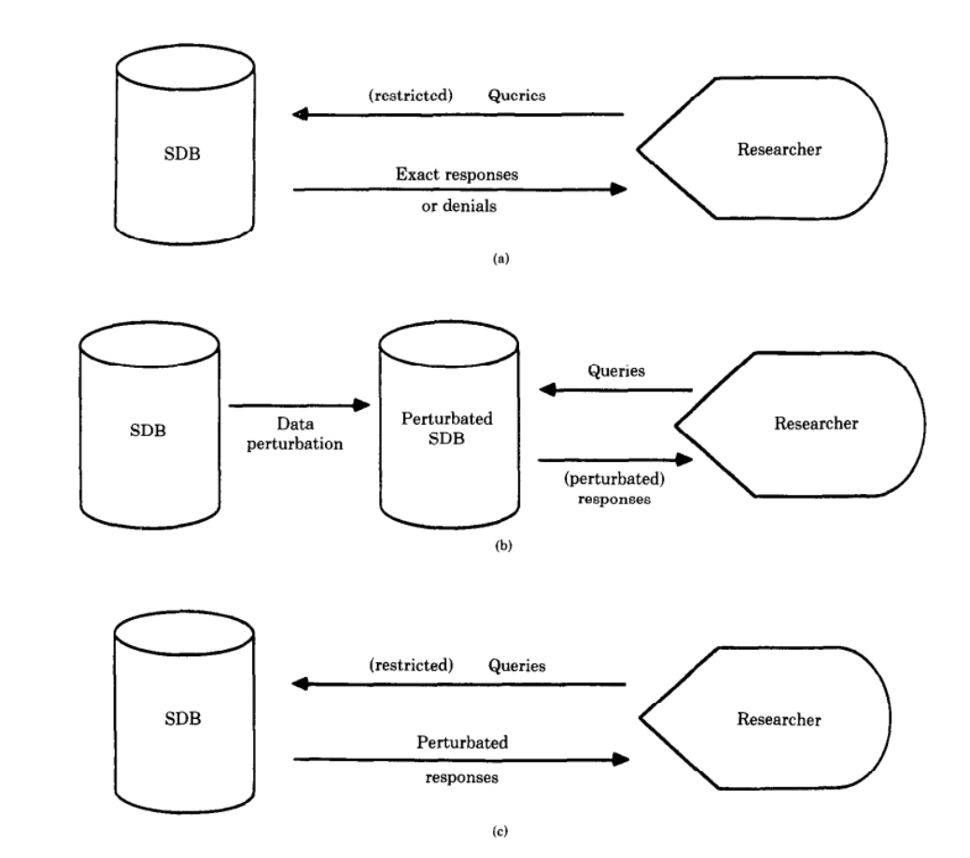
\includegraphics[width=1\linewidth]{assets/text.png}
\caption{Схемы безопасности СБД}
\label{fig:SDB_secure}
\end{figure}


\subsection{Критерии безопасности статистических баз данных}

Критерии безопасности включают оценку вероятности раскрытия записей в СБД, оценку консистентности данных при использовании методов возмущения данных и оценку зависимости между возмущением и конкретными записями. Также учитываются затраты, связанные с выполнением запросов, и назначается конкретная цена каждому запросу. Пользователям предоставляется начальная сумма, которую они могут использовать для запросов, чтобы предотвратить выведение данных.
\\

Когда речь идет о критериях безопасности, необходимо отметить, что полной гарантии безопасности в статистических базах данных (СБД) достичь невозможно. Вместо этого проводится оценка важности деанонимизированных данных и статистической точности, учитывая предпринятые меры по защите данных.
\\

Критерий безопасности \enquote{Security} оценивает вероятность раскрытия (включая частичное раскрытие) записи в СБД. Для каждого разрешенного агрегирующего запроса проводится оценка критерия безопасности. Основываясь на количестве информации в базе данных, можно определить, сколько запросов требуется для деанонимизации данных. На основе этой оценки определяется минимальный размер выборки для таких запросов.
\\

Критерий безопасности \enquote{Consistency} оценивает консистентность данных для методов возмущения данных. Оценивается степень возмущения данных путем создания агрегирующего запроса и измерения его изменений после внесения возмущений. 
\\

Критерий безопасности \enquote{Robustness} оценивает зависимость между возмущением и конкретными записями. Желательно, чтобы возмущение не зависело от данных, однако необходимо сохранить статистические свойства данных.
\\

Критерий безопасности \enquote{Costs} определяет конкретную стоимость каждого запроса. Пользователю предоставляется начальная сумма, которую он может использовать для запросов, чтобы предотвратить вывод данных. Этот критерий скорее представляет собой метод управления, а не непосредственный критерий безопасности.
\\

Таким образом, применение критериев безопасности в СБД позволяет оценивать уровень безопасности, учитывая важность данных, статистическую точность, консистентность, робастность и стоимость запросов.
\\

Исходя из вышеизложенных глав, можем убедиться, что безопасность статистических баз данных является сложной задачей, но существуют различные подходы и методы для обеспечения безопасности данных. Каждый подход имеет свои преимущества и недостатки, и выбор методов безопасности должен основываться на анализе конкретных требований и контекста использования СБД. Оценка важности данных, статистической точности и затрат помогает принять решение о применении конкретных методов обеспечения безопасности.
